%! Author = borisdeletic
%! Date = 12/05/2023

% Preamble
\documentclass[11pt]{article}

% Document
\begin{document}

\section{Performance}\label{sec:performance}
    We aim to showcase the performance strength of our algorithm as a high dimensional sampler compared to existing
    solutions such as PolyChord~\cite{Handley_2015}.
    It is important to note that other samplers do not require the use of gradients unlike CHMC, and can be used for
    likelihoods where no analytic gradient exists, or auto differentiation~\eqref{sec:autodiff} fails.

    A significant advantage of CHMC is that the number of likelihood \& gradient evaluations to generate a sample is
    completely independent of dimension.
    It is defined by the path length alone such that number of calls is $N_{\mathcal{L}, \nabla} = L$ per iteration.
    This means all the dimensionality scaling comes from increasing $n_{\text{live}}$ in order to capture topological
    features of the likelihood, leading to longer convergence times.

    For certain well-behaved likelihoods, it is not even necessary to scale $n_{\text{live}} \sim D$ as suggested by
    Handley et al~\cite{Handley_2015} as shown in the results~\eqref{sec:numerical_results} where $D \gg n_{\text{live}}$.
    Therefore, all the added computational expense comes from longer likelihood evaluation times for more parameters.
    We demonstrate this fact by measuring the average time per sample over a nested sampling run, for a range of
    dimensions up to $D = 1,000,000$.

    \begin{figure}[t!]
        \center
        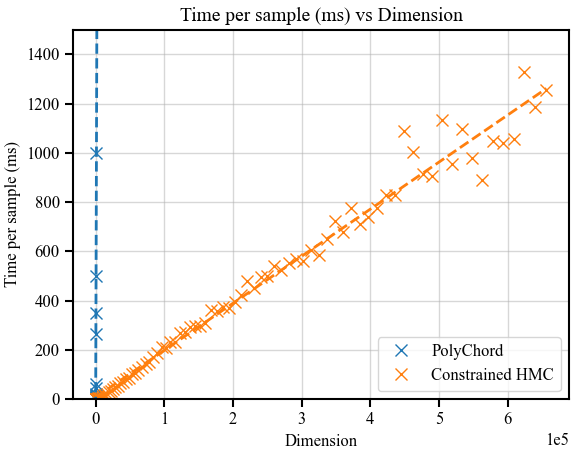
\includegraphics[width=\linewidth]{../figures/Performance}
        \caption{
            64x64 lattice correlation functions.
        }\label{fig:performance}
    \end{figure}

    We also compare the speed per sample using identical setups between PolyChord and our algorithm, shown below.

    For high-dimensional problems, it is clear that the added complexity of using gradients for CHMC is well worth the
    performance benefits.

\end{document}